
%(BEGIN_QUESTION)
% Copyright 2006, Tony R. Kuphaldt, released under the Creative Commons Attribution License (v 1.0)
% This means you may do almost anything with this work of mine, so long as you give me proper credit

Calculate the output voltage of this bridge circuit at the following RTD temperatures (assume the use of a 100 $\Omega$ RTD with a European alpha value).

$$\includegraphics[width=15.5cm]{i00410x01.eps}$$

\begin{itemize}
\item{} $V_{out}$ = \underbar{\hskip 50pt} at $T$ = 0$^{o}$ C
\vskip 5pt
\item{} $V_{out}$ = \underbar{\hskip 50pt} at $T$ = 35$^{o}$ C
\vskip 5pt
\item{} $V_{out}$ = \underbar{\hskip 50pt} at $T$ = $-15^{o}$ C
\end{itemize}

\vskip 20pt \vbox{\hrule \hbox{\strut \vrule{} {\bf Suggestions for Socratic discussion} \vrule} \hrule}

\begin{itemize}
\item{} The low voltage (50 mV) of the ``excitation'' source is not arbitrary, but rather serves a practical purpose.  Explain why it is important for this voltage source to be small in magnitude rather than large (e.g. 5 volts or 24 volts).
\item{} Suppose the only DC voltage source we had available for powering the RTD bridge was a fixed 24 volt source.  How could we make this source work with the bridge circuit shown without encountering problems by over-powering the bridge?
\item{} Choose a resistor at random in this circuit and imagine that it fails (either open or shorted).  Would this electrical fault make the RTD appear hotter than it really is, or colder than it really is?  Explain your answer in detail.
\end{itemize}

\underbar{file i00410}
%(END_QUESTION)





%(BEGIN_ANSWER)

\noindent
{\bf Partial answer:}

\begin{itemize}
\item{} $V_{out}$ = 0.000 mV at $T$ = 0$^{o}$ C
\vskip 5pt
\item{} $V_{out}$ = 1.578 mV at $T$ = 35$^{o}$ C
%\vskip 5pt
%\item{} $V_{out}$ = -0.7433 mV at $T$ = -15$^{o}$ C
\end{itemize}

%(END_ANSWER)





%(BEGIN_NOTES)

\begin{itemize}
\item{} $V_{out}$ = 0.000 mV at $T$ = 0$^{o}$ C
\vskip 5pt
\item{} $V_{out}$ = 1.578 mV at $T$ = 35$^{o}$ C  ($R_{RTD}$ = 113.475 $\Omega$)
\vskip 5pt
\item{} $V_{out}$ = $-0.7433$ mV at $T$ = $-15^{o}$ C  ($R_{RTD}$ = 94.225 $\Omega$)
\end{itemize}


%INDEX% Measurement, temperature: RTD

%(END_NOTES)


